\documentclass[a4paper,12pt]{article}

\usepackage{fontspec}
\usepackage{graphicx}
\usepackage{geometry}
\usepackage{listings}
\usepackage[dvipsnames, svgnames, x11names]{xcolor}
\usepackage{fontspec}
\usepackage{mathtools}
\usepackage{verbatim} 
\usepackage{array}
\usepackage{amsthm}
\usepackage{fancyhdr}
\usepackage{minted}
\usepackage{verbatim}
\usepackage{pdfpages}
\usepackage{enumitem}
\usepackage{setspace}
\usepackage{subfigure}
\usepackage{colortbl}
\usepackage{indentfirst}
\usepackage{titletoc} 
\usepackage{zhnumber}
\usepackage[colorlinks=true]{hyperref}
\usepackage[BoldFont,SlantFont,CJKchecksingle]{xeCJK}

\geometry{left=1.5cm,right=1.5cm,top=1.5cm,bottom=1.5cm}
\setminted[c]{linenos, framesep=2mm, baselinestretch=1.0, breaklines, mathescape, bgcolor=AliceBlue}
\setminted[c++]{linenos, framesep=2mm, baselinestretch=1.0, breaklines, mathescape, bgcolor=AliceBlue}
\setminted[python]{linenos, framesep=2mm, baselinestretch=1.0, breaklines, mathescape, bgcolor=LavenderBlush1}
\setminted[bash]{linenos, framesep=2mm, baselinestretch=1.0, breaklines, mathescape, bgcolor=LavenderBlush1}
\usemintedstyle{color}
\linespread{1.3}

% 中文编号
\renewcommand{\thesection}{\zhnum{section}}
\renewcommand{\thesubsection}{\arabic{section}.\arabic{subsection}}

\setCJKmainfont{SimSun}      % macOS: Songti SC, Windows: SimSun

\begin{document}

\setitemize[1]{itemsep=0pt,partopsep=0pt,parsep=\parskip,topsep=5pt}

% title page
\newgeometry{top=5cm, bottom=5cm}
\thispagestyle{empty}
\begin{center}
    
\includegraphics[width=8cm]{images/logo.jpg}
    \vspace{3em}
    \par\fontsize{30pt}{\baselineskip}\selectfont \textbf{实 \hspace{10pt} 验 \hspace{10pt} 报 \hspace{10pt} 告}
    \large
    \setlength\extrarowheight{2mm} 
    \par\vspace{6em}
    \begin{tabular}{rc}
        \textbf{课\hspace{24pt}程}:& 操作系统原理 \\
        \cline{2-2}
        \textbf{实验标题}:&  体验 nachos 下的并发程序设计 \\
        \cline{2-2}
        \textbf{专\hspace{24pt}业}: & 计算机科学与技术 \\
        \cline{2-2}
        \textbf{时\hspace{24pt}间}: & 2021/3/18 - 2021/4/15 \\
        \cline{2-2}
    \end{tabular}
\end{center}
\restoregeometry

% table of contents
\thispagestyle{empty}
\hypersetup{
    colorlinks=true,
    linkcolor=black
}
\renewcommand\contentsname{\Huge\centering 目\hspace{2em}录\vspace{1em}}
\tableofcontents
\newpage
% main

%% title and author
\setcounter{page}{1}
\begin{center}
    \par \Large \textbf{实验一 · 体验 nachos 下的并发程序设计}
    \vspace{1em}
\end{center}

\normalsize
\par \textbf{实验时间} 2021/3/18 - 2021/4/15
\vspace{0.5em}
\par \textbf{组员}
\vspace{2em}

\section{实验目的}
\par 本次实验的目的在于对 nachos 进行熟悉,并初步体验 nachos 下的并发程序设计。实验内容分三部分:
\begin{itemize}
    \item 安装 nachos,并阅读源代码
    \item 用 C++ 实现双向有序链表
    \item 体验 nachos 线程系统,在 nachos 系统中使用所写的链表程序并演示一些并发错误
\end{itemize}

\section{实验内容及步骤}
\subsection{安装 nachos,阅读源代码}
\par\textbf{Q. 我需要修改/新增 nachos 哪一部分的代码?我不该随意改动哪些代码?}
\begin{itemize}
    \item 可以修改 \mintinline{c++}{#define} 确定机器或者系统参数的指令(比如,物理内存或者默认堆栈的大小);
    \item 可以修改一些测试函数的代码,如本实验中 \mintinline{c++}{ThreadTest} 函数等。
    item 不该修改实现机器本身的任何代码。
\end{itemize}

\par\textbf{Q. code文件夹下的子目录都放了啥? 输入“make depend”、 “ make”、和“./nachos” 都发生了什么? }
\begin{itemize}
    \item code文件夹里面存放了 bin、machine、network 等等文件夹以及 Makefile.common、Makefile、Makefile.dep 文件;
    \item 当输入 make depend 的时候,编译器会自动根据Makefile文件里面的内容形成各个头文件以及c文件的依赖关系;
    \item 当输入 make 的时候,编译器对已经形成依赖关系的文件进行编译,生成可执行文件nachos;
    \item 当输入./nachos 的时候,可执行文件运行。
\end{itemize}

\par\textbf{Q.  我如何 Debug nachos 代码?}
\begin{itemize}
    \item  在代码中添加 printf(或者fprintf)
    \item 使用 gdb 调试器或者其他调试器
    \item 插入对 Nachos 提供的DEBUG函数调用
\end{itemize}

\par\textbf{Q. 如何在 nachos 进行 context switch? }
\begin{itemize}
    \item 在代码中使用 \mintinline{c++}{currentThread->Yield();} 完成强行线程切换
    \item 使用具有 -rs 标志的非自愿上下文切换
\end{itemize}

\par\textbf{Q. nachos 中线程的概念(用户级线程还是内核级线程?)及其运行方式?}
\par 用户级线程,是指用户程序自行采用线程管理库,在应用本身实现线程管理功能;这样的线程是操作系统不可感知的;而内核级线程是由操作系统来管理的。在 nachos 中的 Thread 内实现了线程相关的管理逻辑,并不需要由用户程序自己实现线程管理,因此 nachos 的线程是内核级线程。

\subsection{用 C++ 实现双向有序链表}

\subsubsection{概述}

\par 本实验需要自行编写三个文件 \mintinline{c++}{dllist.h},\mintinline{c++}{dllist.cc} 和 \mintinline{c++}{dllist-driver.cc}。这三个文件的作用说明如下:
\begin{itemize}
    \item dllist.h :由 nachos 的英文文档给出,定义了 DLLElement 类(表示链表节点)和 DLList 类(表示链表本身);本实验需要实现这两个类中定义的方法。
    \item dllist.cc :包含 dllist.h 中定义的 DLLElement 和 DLList 类各方法的实现代码。
    \item dllist-driver.cc :包含了两个工具函数 
    \begin{itemize}
        \item \mintinline{c++}{PutItem(list, N, threadNumber)} :向双向链表中插入随机的 N 个元素
        \item \mintinline{c++}{RemoveItem(list, N, threadNumber)}:连续从双向链表首部删除 N 个元素
    \end{itemize}
\end{itemize}

\subsubsection{Makefile 修改}
\par nachos 使用 Makefile 来管理编译依赖、编译链接规则等。由于本实验中向 nachos 项目中添加了新的三个源码文件,为了让它们能被正常编译链接、并与 nachos 结合,这里需要修改关于 threads 子目录的编译规则,该规则位于 nachos 项目根目录的 Makefile.common 中(这个文件定义了需要使用 gcc 编译的文件,和每个可执行文件需要链接的链接文件)。具体地,需要修改此文件的这些内容:
\begin{itemize}
    \item 在 THREAD\_C 中,添加源代码文件 dllist.cc 和 dllist-driver.cc:
\end{itemize}
\begin{center}
    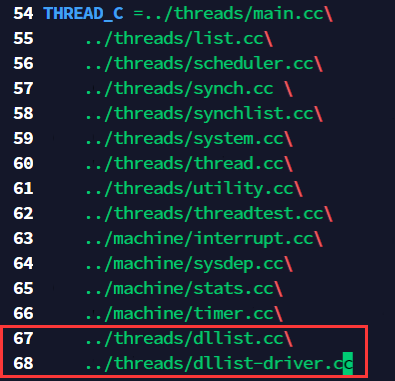
\includegraphics[width=6cm]{images/result/1.png}
\end{center}

\begin{itemize}
    \item 在 THREAD\_H 中,添加头文件 dllist.h:
\end{itemize}
\begin{center}
    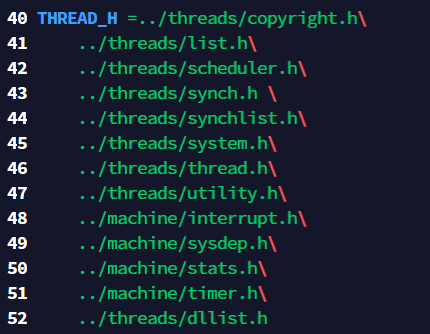
\includegraphics[width=6cm]{images/result/2.png}
\end{center}

\begin{itemize}
    \item 在 THREAD\_O 中,添加由 dllist.cc 和 dllist-driver.cc 编译后产生的链接文件 dllist.o 和 dllist-driver.o:
\end{itemize}
\begin{center}
    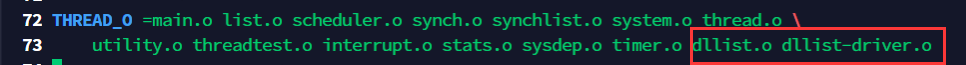
\includegraphics[width=16cm]{images/result/3.png}
\end{center}

\par 完成后,输入 \mintinline{bash}{make depend && make} 指令,检查是否正常重新生成可执行文件。

\subsubsection{代码实现及说明}

\addcontentsline{toc}{subsubsection}{\hspace{1em}dllist.cc}
\par \textbf{dllist.cc}

根据题目的要求,我们需要使用 C++ 实现一个双向链表,而 dllist.h 中已经给出了类定义和方法定义。具体地,我们需要在 dllist.cc 中实现的方法、这些方法的作用及实现思路阐述如下:

\begin{itemize}
\item \mintinline{c++}{DLLElement(void *itemPtr, int sortKey)} :DLLElement 类的构造函数
\par \textbf{实现思路}:简单将 item, key 设置为参数给定的值,然后设置指向 prev, next 为 NULL 即可。
\item \mintinline{c++}{DLList::DLList(), DLList::~DLList()}:DLList 类的构造函数和析构函数
\par \textbf{实现思路}:
\begin{itemize}
  \item 在构造函数中,初始化 first, last 指针为 NULL;
  \item 在析构函数中,将链表中的所有元素 DLLElement 析构,然后将 first, last 设置为 NULL。
\end{itemize}
\item \mintinline{c++}{void DLList::Prepend(void *item)}:在双向链表的首部插入值为 item 的元素,并自动为新元素分配一个小于链表首部原有元素的 key 值的 key 值。
\par \textbf{实现思路}:
\begin{itemize}
  \item 如果双向链表为空即 first == NULL,则创建一个 key 值为 0 的元素,并将指针赋给 first, last。
  \item 否则,创建元素;为了保证 key 的有序性,将新元素的 key 设为 first->key - 1,然后修改新元素的 next 指向和 first 指针的 prev 指向,最后更新 first 指针。
\end{itemize}
\item \mintinline{c++}{void DLList::Append(void *item)}:在双向链表的尾部插入值为 item 的元素,并自动为新元素分配一个大于链表尾部原有元素的 key 值的 key 值。
\par \textbf{实现思路}:同上,将上面插入到首部的步骤对偶即可。
\item \mintinline{c++}{void* DLList::Remove(int *keyPtr)}:从双向链表的头部删除一个元素,并将被删除元素的 key 值传给参数指针。
\par \textbf{实现思路}:将 first 指向 first->next,然后将原先的 first 指向的元素析构即可。
\item \mintinline{c++}{bool DLList::IsEmpty()}:当双向链表不为空时,返回 true
\par \textbf{实现思路}:当 first == last == NULL 时,表示双向链表为空。
\item \mintinline{c++}{void DLList::SortedInsert(void *item, int sortKey)}:将 key 值为 sortKey 的元素插入到双向链表的正确位置中。
\par \textbf{实现思路}:
\begin{itemize}
  \item 如果链表为空,直接插入到首部并修改 first, last 的指向
  \item 否则,从 first 开始遍历链表,直到找到 x->key > key 的元素 x 或找不到这样的元素为止。
    \item 如果找不到这样的元素,即链表中所有元素的 key 都比给定的 key 少,则将其插入到表尾,修改 last->next 和 newElement->prev,然后修改 last 的指向。
    \item 如果找到了元素 x,则更新 newElement->prev, newElement->next, x->next->prev 和 x->next。
\end{itemize}
\item \mintinline{c++}{void* DLList::SortedRemove(int sortKey)}:删除 key 值为 sortKey 的元素(如果存在)。
\par \textbf{实现思路}:从首部遍历,找到符合条件的节点,修改该节点前、后节点的连接关系即可。
\end{itemize}

\par 具体代码实现如下:
\begin{minted}{c++}
#include "stdio.h"
#include "stdlib.h"
#include "assert.h"
#include "dllist.h"
#include "thread.h"

extern Thread *currentThread;

// initialize a list element (constructor, destructor)
DLLElement::DLLElement(void *itemPtr, int sortKey)
{
    item = itemPtr;
    key = sortKey;
    next = NULL;
    prev = NULL;
}

DLList::DLList()
{
    first = NULL;
    last = NULL;
}

// in destructor function, we delete all DLLElement(s) in the current list
// and set first/last pointer to NULL
DLList::~DLList()
{
    DLLElement *ptr;
    while (first != NULL) {
        ptr = first;
        first = first->next;
        delete ptr;
    }
    last = NULL;
}

// add to head of list, set key = min_key - 1
void DLList::Prepend(void *item)
{
    DLLElement *curItem = new DLLElement(item, (first == NULL) ? 0 : (first->key - 1));
    curItem->next = first;
    if (first != NULL)
        first->prev = curItem;
    first = curItem;
    last = (last == NULL) ? curItem : last;
}

// add to tail of list, set key = max_key + 1
void DLList::Append(void *item)
{
    DLLElement *curItem = new DLLElement(item, (last == NULL) ? 0 : (last->key + 1));
    curItem->prev = last;
    if (last != NULL)
        last->next = curItem;
    last = curItem;
    first = (first == NULL) ? curItem : first;
}

// remove from head of list
// set *keyPtr to key of the removed item
// return item (or NULL if list is empty)
void* DLList::Remove(int *keyPtr)
{
    if (first == NULL)
        return NULL;
    *keyPtr = first->key;
    DLLElement *removedItem = first;
    last = (first == last) ? NULL : last;
    first = first->next;
    if (first != NULL)
        first->prev = NULL;
    return removedItem;
}

// return true if list has elements
bool DLList::IsEmpty()
{
    return (first != NULL && last != NULL);
}

// routines to put/get items on/off list in order (sorted by key)
void DLList::SortedInsert(void *item, int sortKey)
{
    if (first == NULL || sortKey <= first->key) {
        Prepend(item);
        first->key = sortKey;
        return;
    }

    DLLElement *newItem = new DLLElement(item, sortKey),
               *ptr = first;
    while (ptr != NULL && ptr->key < sortKey)
        ptr = ptr->next;
    if (ptr == NULL) {
        last->next = newItem,
        newItem->prev = last,
        last = newItem;
    }
    else {
        ptr->prev->next = newItem,
        newItem->prev = ptr->prev,
        newItem->next = ptr,
        ptr->prev = newItem;
    }
}

void* DLList::SortedRemove(int sortKey)
{
    DLLElement *ptr = first;
    assert(first != NULL);
    while (ptr != NULL && ptr->key < sortKey)
        ptr = ptr->next;
    if (ptr == NULL || ptr->key != sortKey)
        return NULL;
    if (ptr->next != NULL)
        ptr->next->prev = ptr->prev;
    if (ptr->prev != NULL)
        ptr->prev->next = ptr->next;
    return ptr->item;
}
\end{minted}

\addcontentsline{toc}{subsubsection}{\hspace{1em}dllist-driver.cc}
\par\textbf{dllist-driver.cc}

\par 根据题目需求,我们还需要实现两个工具函数,其中一个函数生成 N 个随机 key 的元素并插入双向链表;另一个函数从链表首部依次移除 N 个元素。具体代码实现如下:

\begin{minted}{c++}
void PutItem(DLList *list, int n, int threadNumber) 
{ 
    if (!isSranded) { 
        isSranded = true; 
        srand(time(NULL)); 
    } 
    for (int i = 0; i < n; i++) { 
        int key = rand() % 1000; 
        printf("[Thread %d] insert: %d\n", threadNumber, key); 
        list->SortedInsert((void*)key, key); 
        list->foreach(0); 
    } 
} 
 
void RemoveItem(DLList *list, int n, int threadNumber) 
{ 
    for (int i = 0, key; i < n; i++) { 
        printf("[Thread %d] remove: ", threadNumber); 
        list->Remove(&key); 
        printf("%d\n", key); 
        list->foreach(0); 
    } 
}
\end{minted}

\addcontentsline{toc}{subsubsection}{\hspace{1em}修改 nachos 的 threadtest.cc 和 main.cc}

\par\textbf{修改 nachos 的 threadtest.cc 和 main.cc}

为了让我们编写的代码能够通过 nachos 运行,需要修改 \textit{main.cc} 和 \textit{threadtest.cc},添加相关的函数调用和运行参数,以便于测试。
首先,对 \textit{threadtest.cc} 做出如下修改:
\begin{itemize}
\item 定义全局变量 \mintinline{c++}{numberCount} 表示每轮次随机生成的数字个数,默认 \mintinline{c++}{numberCount = 10}.
\item 添加两个函数 \mintinline{c++}{ThreadTest2()} 和 \mintinline{c++}{DLListThread()} 作为测试的入口。
\end{itemize}
为了下一部分实验的方便,在这里同时做了以下事情:
\begin{itemize}
\item 定义全局变量 \mintinline{c++}{threadNum} 表示同时运行的线程数。
\item 在 \mintinline{c++}{ThreadTest2()} 中实现线程的创建和运行。    
\end{itemize}

\begin{minted}{c++}
void DLListThread(int threadNum) 
{ 
    PutItem(list, numberCount, threadNum); 
    RemoveItem(list, numberCount, threadNum); 
} 
 
 
void ThreadTest2() 
{ 
    DEBUG('t', "Entering ThreadTest2"); 
 
    DEBUG('t', "Creating DLList()"); 
    list = new DLList(); 
 
    DEBUG('t', "Creating fork thread"); 
    for (int i = 1; i < threadCount; i++) { 
        Thread *t = new Thread("fork thread"); 
        t->Fork(DLListThread, i); 
    } 
 
    DLListThread(0); 
 
    if (list != NULL) 
        delete list;
}
\end{minted}

\par 然后在 \textit{main.cc} 中,添加自定义参数。nachos 已经预定义了一部分参数,如 -q 用于指定测试的编号。这里再添加 -n 参数用于指定 \mintinline{c++}{numberCount}:

\begin{minted}{c++}
for (argc--, argv++; argc > 0; argc -= argCount, argv += argCount) { 
    argCount = 1; 
 
    switch (argv[0][1]) { 
    case 'q': 
        testnum = atoi(argv[1]); 
        argCount++; 
        break; 
    case 'n': 
        numberCount = atoi(argv[1]); 
        argCount++; 
        break; 
    case 't': 
        threadCount = atoi(argv[1]); 
        argCount++; 
    default: 
        break; 
    } 
} 
\end{minted}

\subsubsection{实现效果}

\par 添加相应的 verbose 函数显示链表的插入和删除过程:

\begin{minted}{c++}
void DLList::foreach(bool showRelation)  
{  
    int sz = 0, flag = 0;  
    DLLElement *ptr = first;  
    printf("\t   ");  
  
    while (ptr != NULL) {  
        flag = 1;  
        if (sz != 0)  
            printf("->");  
        printf("%d", ptr->key);  
        if (showRelation) {  
            printf("(");  
            if (ptr->prev != NULL)  
                printf("p=%d", ptr->prev->key);  
            if (ptr->prev != NULL && ptr->next != NULL)  
                printf(" ");  
            if (ptr->next != NULL)  
                printf("n=%d", ptr->next->key);  
            printf(")");  
        }  
        sz++, ptr = ptr->next;  
    }  
    if (flag)  
        putchar(' ');  
    printf("(total: %d)\n", sz);  
}
\end{minted}

\par 然后执行 make 命令编译新的 nachos 可执行文件,执行命令:

\begin{minted}{bash}
./nachos -q 2 -t 1 -n 5   # 运行 ThreadTest2, 单线程运行,每轮次生成 5 个数字
\end{minted}

\par 效果如下:
\begin{center}
    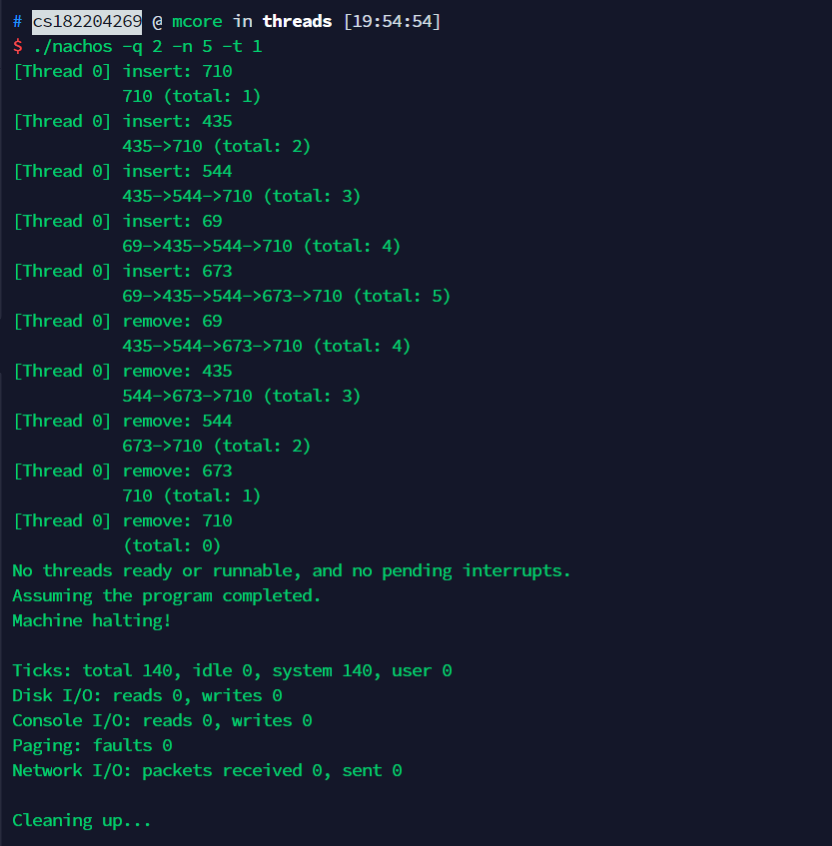
\includegraphics[width=12cm]{images/result/4.png}
\end{center}

\subsection{体验 nachos 线程系统}
\subsubsection{实验任务}
修改Nachos源代码体验并发程序问题 :

\begin{itemize}
\item 修改 \textit{nachos-3.4/code/threads/threadtest.cc} 和 \textit{nachos3.4/code/threads/main.cc},重新编译 threads 子系统,使得链表操作可以在 Nachos 中运行并实现用两个线程并发操作链表。 
\item 自行设计可能使并发链表操作发生错误的线程执行顺序,考虑3-5 种不同的顺序为宜; 
\item 实现以上执行顺序:修改 \textit{nachos3.4/code/threads/threadtest.cc} ,在“适当”的位置(使得可以观察到并发程序问题)插入 \mintinline{c++}{currentThread->Yield()} 调用以强制线程切换,重新编译 threads 子系统并运行观察出现的问题。     
\end{itemize}

\subsubsection{实验设计}
\addcontentsline{toc}{subsubsection}{期望结果}
\par \textbf{\hspace{1em}期望结果}
\par 在此任务中,我们假定程序拥有两个线程 Thread 0 和 Thread 1,分别执行链表的顺序插入和首部删除操作各 5 次。
\par 为了下文说明的便利,我们期望两个线程正确的执行顺序如下:
\begin{itemize}
\item Thread 0 和 Thread 1 默认交替执行插入和删除操作。
\item 任一线程执行插入操作 PutItem 时,总是随机生成一个数插入到链表中的对应位置,分配空间并维护节点链接;插入操作完成后,才切换至另一线程;
\item 任一线程执行删除操作 RemoveItem 时,总是删除链表首部(最小)的元素,维护节点链接和表头指向,然后将被删除的节点析构 (delete);删除操作完成后,才切换至另一线程。   
\end{itemize}

\par 因此,我们期望的运行结果应如下图所示:
\begin{center}
    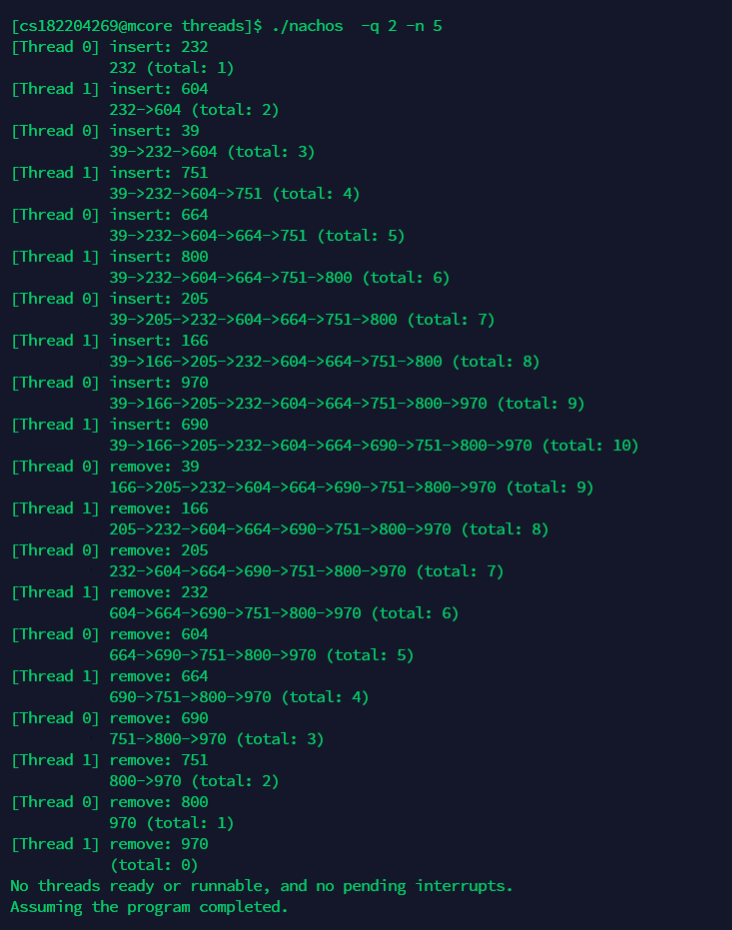
\includegraphics[width=10cm]{images/result/5.png}
\end{center}

\addcontentsline{toc}{subsubsection}{执行顺序设计}
\par\textbf{\hspace{1em}执行顺序设计}
\par 上文所提到的正确执行顺序,都是建立在 “插入操作和删除操作都是原子操作” 的前提之下的;然而,在实际的情况中并不是这样。具体地说,插入操作可以被分为以下几个阶段:
\begin{itemize}
\item 创建 DLLElement 对象 (new)
\item 寻找插入位置,并设置新节点的相邻指向
\item 修改前、后节点的相邻指向
\item 维护表头/表尾
\end{itemize}

\par 而表头删除操作可以被分为以下几个阶段:
\begin{itemize}
\item 修改被删除节点的相邻节点的 prev 指向
\item 维护表头/表尾
\item 析构被删除的节点(delete)    
\end{itemize}

\par 如果在上述每个阶段的之间,执行线程的切换,则这样的 “错误执行顺序” 可能就会引发错误的结果,例如:
\begin{itemize}
\item Thread 0 在插入节点、修改相邻指向的阶段时,Thread 1 在当前节点的附近位置插入一个新节点。
\item Thread 0 插入了一个最小的元素、在修改表头的指向的阶段时,Thread 1 从表头删除了元素。
\item Thread 0 和 Thread 1 同时从表头删除了一个元素。    
\end{itemize}

\subsubsection{代码实现、说明及效果}

\addcontentsline{toc}{subsubsection}{\hspace{1em}Case 1: 同时向表头插入一个最小的元素,导致其中一个元素未被成功插入}
\par\textbf{Case 1: 线程 0 和 线程 1 同时向表头插入一个最小的元素,导致其中一个元素未被成功插入}

此场景模拟如下:

\begin{minted}{text}
- 表头 first 指向节点 node0 对应的 key 为 a
- 线程 0 创建了一个 DLLElement 对象 node1,设置其 key 为 b (b < a)
- 线程 0 将 first->prev 赋值为 node1
- 发生线程切换
- 线程 1 创建了一个 DLLElement 对象 node2,设置其 key 为 c (c < b)
- 此时 first 指针尚未被赋值为 node1,线程 1 将 first->prev 赋值为 node2
- 发生线程切换
- 线程 0 将 first 赋值为 node1
- 发生线程切换
- 线程 1 将 first 赋值为 node2
- 发生线程切换

期望结果:node2(c) -> node1(b) -> node0(a), first = node2
实际结果:node2(c) -> node0(a), first = node2
结果对比:node1 未能成功插入链表
\end{minted}

\par 为了实现这种执行顺序,在每次向首部插入元素、修改 first 指针之前,调用 \mintinline{c++}{currentThread->Yield()}:

\begin{minted}{c++}
// add to head of list, set key = min_key - 1 
void DLList::Prepend(void *item) 
{ 
    DLLElement *curItem = new DLLElement(item, (first == NULL) ? 0 : (first->key - 1)); 
    curItem->next = first; 
    if (first != NULL) 
            first->prev = curItem; 

    // 执行强制线程切换
    if (threadTestcase == 1) 
            currentThread->Yield(); 

    first = curItem; 
    last = (last == NULL) ? curItem : last; 
}
\end{minted}

\par 运行结果如图所示。当两个线程同时往链表首部插入元素时,错误的执行顺序会导致其中一个插入的数丢失;而如果在不同的位置插入,则不会发生此问题。
\begin{center}
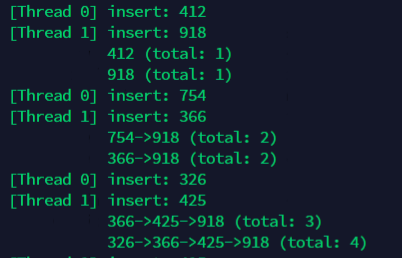
\includegraphics[width=8cm]{images/result/6.png}
\end{center}

\addcontentsline{toc}{subsubsection}{\hspace{1em}Case 2: 在同一位置插入元素,导致链表 Key 有序性被破坏}
\par \textbf{Case 2: 线程 0 和线程 1 在同一位置插入元素,导致链表 Key 有序性被破坏}
\par 此场景模拟如下:

\begin{minted}{text}
- 初始化链表,插入 key 为 1 的节点 node1、key 为 4 的节点 node4
- 线程 0 创建了一个 DLLElement 对象 node3,设置其 key 为 3
- 线程 0 找到节点插入位置为 node4 之前
- 发生线程切换
- 线程 1 创建了一个 DLLElement 对象 node2,设置其 key 为 2
- 由于尚未修改关联,线程 1 找到节点插入位置为 node4 之前
- 发生线程切换
- 线程 0 修改:
-        node3->prev = node1
-        node3->next = node4
-        node1->next = node3
-        node4->prev = node3
- 发生线程切换
- 线程 1 修改:
-        node2->prev = node1
-        node2->next = node4
-        node1->next = node2
-        node4->prev = node2

期望结果:node1(1) -> node2(2) -> node3(3) -> node4(4)
实际结果:node1(1) -> node3(3) -> node2(2) -> node4(4)
结果对比:后插入的 node2 本来应该被插入到 node3 之前,但由于关联未修改导致失序
\end{minted}

\par 为了实现这种执行顺序,手动插入元素 1, 4 后执行 \mintinline{c++}{t->Fork();} ,然后分别在线程中,先后插入 3, 2.
\par 同时对插入元素对应位置做出修改:

\begin{minted}{c++}
void DLList::SortedInsert(void *item, int sortKey) 
{ 
        if (first == NULL || sortKey <= first->key) { 
                Prepend(item); 
                first->key = sortKey; 
                return; 
        } 
 
        DLLElement *newItem = new DLLElement(item, sortKey), 
                           *ptr = first; 
        while (ptr != NULL && ptr->key < sortKey) 
                ptr = ptr->next; 
        if (ptr == NULL) { 
                last->next = newItem, 
                newItem->prev = last, 
                last = newItem; 
        } 
        else { 
                // 找到插入位置后,进行强制线程切换
                if (threadTestcase == 2) 
                        currentThread->Yield(); 
                ptr->prev->next = newItem; 
                newItem->prev = ptr->prev; 
                newItem->next = ptr; 
                ptr->prev = newItem; 
                if (threadTestcase == 2) 
                        currentThread->Yield(); 
        } 
}
\end{minted}

\par 运行结果如图所示:
\begin{center}
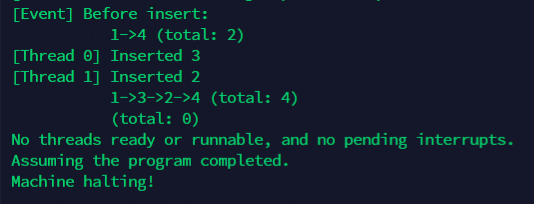
\includegraphics[width=9cm]{images/result/7.png}
\end{center}

\addcontentsline{toc}{subsubsection}{\hspace{1em}Case 3: 同时向表头插入元素和删除元素,导致删除了非表头元素}
\par\textbf{Case 3: 线程 0 向表头插入元素,线程 1 同时从表头删除元素,导致删除了非表头元素}
\par 此场景模拟如下:
\begin{minted}{text}
- 初始时,链表有序非空,表头元素为 node0 (key = a) -> node1
- 线程 0 创建了一个 DLLElement 对象 node2 设置 key = b (b < a)
- 线程 0 修改了 node2->next
- 发生线程切换
- 线程 1 删除了表头元素 node0
- 线程 1 修改了 node0->next->prev 和 first 指针
- 线程 1 析构 (delete) 了 node0
- 发生线程切换
- 线程 0 修改 first 指针指向 node2

期望结果:node0(a) -> node1 -> ...
实际结果:node2(b) -> NULL
                                    node1 -> ...
结果对比:线程 1 后执行删除操作,但删除的却不是表头的元素;同时破坏了链表的连续性。
\end{minted}

\par Case 3 和 Case 1 在切换线程的位置是相同的。不同的是,Case 3 手工构造了插入的顺序。运行结果如图所示:
\begin{center}
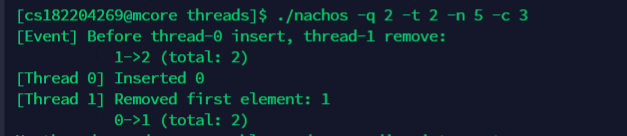
\includegraphics[width=10cm]{images/result/8.png}
\end{center}

\addcontentsline{toc}{subsubsection}{\hspace{1em}Case 4: 同时删除表头元素,由于节点已被析构导致段错误}
\par\textbf{Case 4: 线程 0 和线程 1 同时删除表头元素,由于节点已被析构导致段错误}
\par 此场景模拟如下:
\begin{minted}{text}
- 初始时,链表有序非空,表头元素为 node0 
- 线程 0 试图删除表头节点,找到 node0
- 发生线程切换
- 线程 1 试图删除表头节点,找到 node0
- 线程 0 设置 first = first->next (NULL)
- 线程 0 将 node 0 析构
- 发生线程切换
- 线程 1 试图设置 first = first->next,但由于此时 first 为 NULL,因此发生段错误

期望结果:NULL
实际结果:Segmentation Fault
\end{minted}

\par 对代码 Remove 函数做出的修改如下:
\begin{minted}{c++}
// remove from head of list 
// set *keyPtr to key of the removed item 
// return item (or NULL if list is empty) 
void* DLList::Remove(int *keyPtr) 
{ 
        if (first == NULL) 
                return NULL; 
        *keyPtr = first->key; 
        // get first remove element 
        DLLElement *removedItem = first; 
 
       // 修改 first 指向前,强制切换线程
        if (threadTestcase == 4) { 
                printf("Prepare to remove: %d\n", first->key); 
                currentThread->Yield(); 
        } 
 
        // set first & last pointer 
        last = (first == last) ? NULL : last; 
        first = first->next; 
        if (first != NULL) 
                first->prev = NULL; 
 
        void* element = removedItem->item; 
        delete removedItem; 
        return element; 
}
\end{minted}

\par 结果如图所示:
\begin{center}
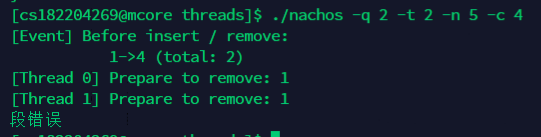
\includegraphics[width=9cm]{images/result/9.png}
\end{center}

\section{实验总结与感想}
\par 通过本次实验,我们简单地阅读了 nachos 的源代码,对 nachos 的工作原理、整体情况,以及如何修改 nachos 的代码实现部分功能,有了初步的了解,并使用 C++ 实现了双向链表在 nachos 上运行测试。尤其是体验了 nachos 的线程机制,并通过实验测试了线程执行顺序的不同,对程序正确性的影响。

\end{document}